\chapter{Uso em Algortimos}

\section{Algortimos Classificatórios}
% 

Algoritmos classificatórios
podem ser lineares ou não lineares. 
Classificadores lineares conseguem separar 
as categorias de dados em uma reta no espaço vetorial, seja ela com uma ou mais dimensões (reta, plano ou hiperplano) (Souza, 2018). Para problemas mais complexos,
é comum o uso de algoritmos que classifiquem dados não lineares, como o \textit{Support Vsector Machine} (SVM), 
\textit{K-Nearest Neightbor} (KNN) e
Rede Neural Artificial (ANN).

Para a avaliação do algoritmo, a acurácia e precisão oferecem métricas para avaliar o erro observado do output (ou resultado) do modelo. 
Para isso, é necessário saber o valor real e o valor estimado pelo algoritmo classificatório. 
A acurácia mede a proximidade de um determinado valor e o valor de referência (ou valor real) (equação 5.1). 
A precisão mede a dispersão dos valores obtidos pelo modelo (equação 5.2). Um bom algoritmo é preciso e possui alta acurácia. 

\begin{equation}
      Accuracy = \frac{TP+TN}{TP+TN+FP+FN}
\end{equation}

\begin{equation}
      Precision = \frac{TP}{TP+FP}
\end{equation}

\begin{equation}
      Recall = \frac{TP}{TP+FN}
\end{equation}

\begin{equation}
      F1 = \frac{2*Precision*Recall}{Precision+Recall} = \frac{2*TP}{2*TP+FP+FN}\text{,}
\end{equation}

onde TP = verdadeiros positivos, ou onde a previsão do valor tido com verdadeiro estava correta; TN = verdadeiros negativos;
FP e FN onde o modelo errou e em qual modalidade (se na classificação dos positivos ou dos falsos, respectivamente).
Por este motivo, existe a necessidade de separar o dataset em dataset de treino e dataset de teste. De forma habitual, o dataset
de teste é 20\% do dataset total, selecionado de forma aleatória. Ao final do momento de treinamento, onde o algoritmo 
tenta encontrar padrões nas diferentes classes do dataset, o dataset de teste é classificado pelo algortimo de acordo 
com o que foi aprendido e então as métricas de performance são calculadas. 


%referencia: Duda, Richard O.; Stork, David G. (2001). Pattern classification 2nd ed ed. New York: Wiley. OCLC 41347061
A performance de algoritmos classificatórios também pode ser observada 
através de uma matriz de confusão (Duda e Stork, 2001).
Esta matriz permite observar onde o algoritmo mais erra - se em 
classificar verdadeiros positivos ou verdadeiros negativos. 

Outra forma de avaliação é através da curva ROC, 
ou Característica de Operação do Receptor. A curva é obtida a
o se observar a variação da taxa de verdadeiros positivos 
(sensibilidade, ou Positivos Verdadeiros / Positivos Totais) em função de 1 – 
especificidade, ou taxa de falsos positivos (Positivos Falsos / Negativos Totais). 

\section{Uso de Datasets Multimodais de EEG e ET na Pesquisa}

Em seu estudo sobre o uso de algoritmos para classificação de emoções a partir de dados fisiológicos, 
Zheng et al. (2014) coletou dados de dilatação da pupila, movimentação ocular e EEG para 
identificar qual seria a classificação do estímulo emocional apresentado aos participantes. 
O processo de coleta do estudo pode ser observado na figura 5.3. 
A classificação do estímulo apresentado (vídeo clips de 4 minutos de duração) 
obteve acurácia máxima de \textbf{73.59\%} de dados coletados em 12 sessões de experimento, 
onde, em cada sessão, os 5 participantes assistiram a 15 vídeos 
(5 de emoção neutra, 5 de positiva e 5 de negativa). 
 

\begin{figure}[!h]
      \centering
      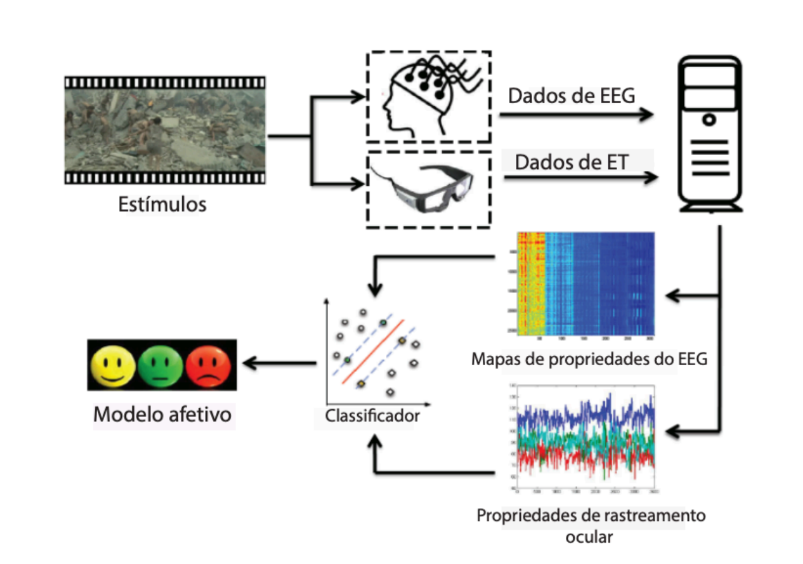
\includegraphics[width=150mm]{estimulo_e_coleta.png}
      \caption{Design de Experimento para Coleta de EEG e ET. Fonte: Zheng et al. (2014)}
\end{figure}

Lu et al. (2015) também faz uso de dados de EEG e ET para classificação de emoções nas três 
valências emocionais eleitas no estudo de Zheng et al. (2014). Em contraste com o volume de 
informações coletadas no estudo de Zheng et al., Lu et al. coletam uma maior quantidade de dados de rastreamento ocular – 
extraindo 16 métricas de ET, enquanto o estudo de Zheng foca em apenas métricas principais da dilatação ocular. 
Os resultados da acurácia do algoritmo aplicado aos diferentes métodos de fusão de dados multimodais estão resumidos na imagem 5.4, 
ficando evidente que, independente do método utilizado para fusão das modalidades de EEG e ET, 
as melhores acurácias foram encontradas para base de dados de mais de uma fonte de informação fisiológica. 

\begin{figure}
      \centering
      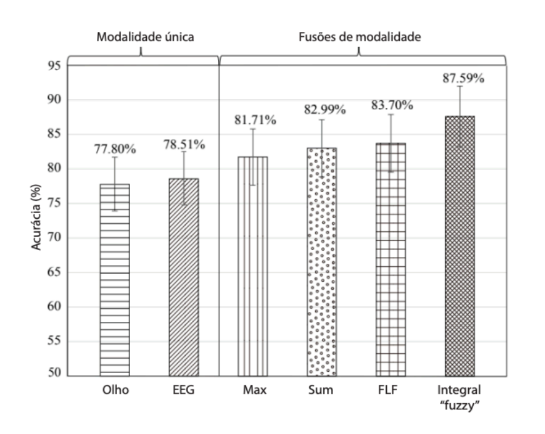
\includegraphics[width=100mm]{lu.png}
      \caption{Acurácia por Método de Fusão de Modalidade e Modalidade Única em Algoritmo Supervisionado. Fonte: Lu et. al. (2015)}
\end{figure}

No trabalho de Thapaliya et al. (2019) dados de EEG e ET foram aplicados em algoritmos de máquina, 
com o objetivo de estudar uma melhora no método de diagnóstico de crianças com autismo através de 
diferentes formas de pré-processamento (exemplo de processamento do estudo na figura 5.5). 
Os dados de EEG tiveram suas métricas estatísticas coletadas para a construção de um vetor de características 
(incluindo desvio padrão e média por janela de tempo dos dados de EEG filtrados), assim como a entropia calculada 
por janela temporal. Para os dados de ET, os tempos de fixação foram coletados, em conjunto com o resultado de testes cognitivos. 
Em seu estudo, diferentes métodos de construção de vetores de características foram analisados, 
tanto para os dados unimodais quanto para a junção de EEG e ET. 
Através das acurácias apresentadas para os diferentes métodos de processamento, 
é possível observar que determinados algoritmos aumentaram sua acurácia a
 depender do modo no qual o vetor de características foi construído. 
 Por exemplo, enquanto o algoritmo Support Vector Machine (SVM) atingiu \textbf{71\%} de acurácia 
 com o vetor que incluiu Entropia para as janelas de EEG e PCA, a regressão logística com maior acurácia 
 foi atingida com o dataset de desvio padrão de EEG e dados de rastreamento ocular sem a aplicação de PCA 
 (Thapaliya et al., 2019). 

Lim e Chia (2015), estudaram a correlação de ondas EEG detectadas em um equipamento de eletrodo único e 
estresse cognitivo induzido pelo teste de Stroop. A análise foi feita com base na aplicação de três algoritmos: 
\textit{Artificial Neural Network}, \textit{k-Nearest Neighboor} (KNN) e \textit{Linear Discriminant Analysis} (LDA), 
dos dados de EEG transformados pela aplicação da Transformação Cosseno Discreta (\textit{Discrete Cosine Transform} – DCT). 
O KNN com o DCT conseguiu classificar melhor o estado de estresse do participante.

\section{Equipamentos Comerciais na Pesquisa}

O uso do MindWave Mobile II foi recentemente empregado para o 
controle de cadeira de rodas (Abuzaher e Al-Azzeh, 2021; Permana et al., 2019), 
controle de mão robótica e robô móvel (Purnamasari et al., 2019; Rusanu et al., 2019; Rușanu et al., 2021) 
e predição de personalidade (Bhardwaj et al., 2021). 

Outro estudo com uso de eletrodo único como fonte de dados eletrofisiológicos foi o trabalho de Quesada-Tabares et al. (2017), 
onde foi demonstrado que o uso de EEG comercial e com eletrodo único também possui um importante poder classificatório 
quando aplicado em algoritmos. Em seu estudo, sete participantes observaram imagens selecionadas do 
\textit{International Affective Picture System} (IAPS) pertencentes a três grupos com diferentes valores de 
valência e excitabilidade. O teste de Análise de Variância aplicado indicou 
uma diferença estatisticamente significante entre os sets de imagens.
 Um segundo teste foi conduzido pela aplicação de um algoritmo de classificação no estilo árvore de decisão,
  chegando a uma acurácia média entre os sete participantes de \textbf{80.71\%}.

Bos (2021) também explora o uso do Mindwave no contexto escolar para medir a atenção dos alunos. Em seu estudo, 
o nível de atenção com alunos assistindo a um vídeo educacional sem e outro com interações (fazendo pergunta aos alunos)
 é explorado e a distribuição percentual das diferentes bandas de frequência são comparadas entre os grupos. Foi 
 observado uma relativa diminuição banda de frequência de onda beta para o grupo que não assistiu ao vídeo interativo, 
 o que foi relacionado a um processamento cognitivo reduzido e menor atenção.


%Bhardwaj et al. (2021) analisou o uso dos dados coletados com o Mindwave para classificar sete traços de personalidade 
%com o algoritmo \textit{deep long short term memory} (DeepLSTM) e tratando os dados com transformada de Fourier Rápida. 
%A pesquisa contou com 50 participantes (25 mulheres e 25 homens), com idades entre 18 e 46 anos, e durou cinco dias.
%Os dados foram coletados enquanto os participantes assistiam vídeos relacionados a traços de personalidade. 
% Os traços foram separados de acordo com os tipos de personalidade definidos no \textit{Myers-Briggs Type Indicator}, 
% e ao final de cada vídeo, o participante deveria dizer se concordava, 
% discordava ou era neutro aos questionários de personalidade sobre o traço proeminente no estímulo. 
% O questionário de cada participante foi utilizado para determinar o traço de personalidade, 
% que serviria para então classificar os dados em três possíveis outputs: 
% (a) participante tem traço de personalidade apresentado no vídeo, (b) participante não tem traço apresentado de forma significativa 
% e (c) participante tem traço oposto ao apresentado no vídeo.
 
% [FALTOU CONCLUSÃO AQUI]


\begin{figure}[h]
      \centering
      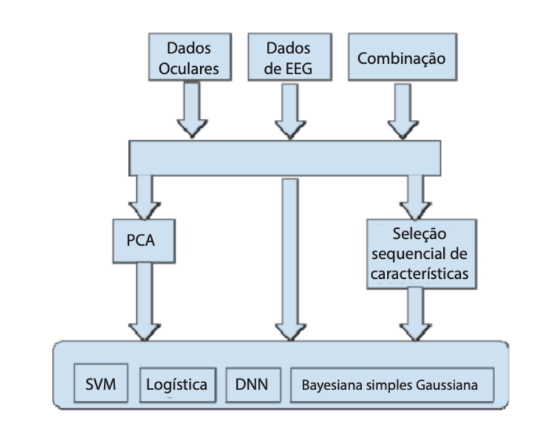
\includegraphics[width=100mm]{thapalya.png}
      \caption{União de dados de EEG e ET. Fonte: Thapaliya et al. (2019)}
\end{figure}

\section{Considerações Finais}
Datasets multimodais tendem a performar melhor em algoritmos classificatórios que datasets unimodais. 
A forma de processamento dos dados também pode ter impactos na performance classificatórias dos algoritmos. 
Equipamentos comerciais já foram previamente utilizados em estudos de algoritmos classificatórios. 
É esperado que um método de tratamento eficiente reflita em uma maior acurácia dos algoritmos treinados no dataset. 

